\documentclass[12pt]{article}

\usepackage{graphicx}
\graphicspath{ {./Fichier_Image/} }

\title{10 Premiers Bâtiments}
\author{Thibault Clodion}

\begin{document}

\maketitle % Permet d'afficher le titre, l'author etc

\section{Type de Batiments}

\begin{itemize}

\item 1. Couloir 1 m
\item 2. Couloir 1.50 m
\item 3. Couloir sans limite
\item 4. 5 Personnes max par bureau
\item 5. 10 Personnes max par bureau
\item 6. 20 Personnes max par bureau
\item 7. 30 Personnes max par bureau
\item 8. Aucune limite de personnes max par bureau
\item 9. 1 Porte par bureau
\item 10. 2 Porte par bureau

\end{itemize}

\underline{Schéma de la forme générale du batiment :}\newline
\includegraphics[scale=0.17]{General Looking.jpg}

\section{Observations}

\begin{itemize}

    \item 2. Temps moyen de dernière sortie : 24.55 sec
    \newline Temps max de dernière sortie : 28.68 sec
    \newline 
    D'abord après 100 simulations on obtient un temps moyen de sortie étant de 24.55 sec.
    Pour le batiment avec les 250 tables uniformes j'avais un temps moyen de 26.20 sec. C'est donc encourageant
    car cela veut dire que la disposition du bâtiment influe effectivement sur le temps de sortie.
    \newline
    Le bâtiment est un peu vide mais on peut déjà constater plusieurs phénomènes intéressant :
    \newline
    $\hspace*{0.2cm}$- L'important est de \textbf{Diviser le flux} cela permet d'évider les "embouteillages"
    \newline
    $\hspace*{0.2cm}$- Il est aussi important de disposer les tables et bureaux loin des "passages" cela permet
    une arrivée plus rapide vers la sortie sans besoin d'esquiver des meubles
    \newline
    $\hspace*{0.2cm}$- Il est très intéressant d'éloigner les portes entres elles. Car les flux sont importants proches
    des portes, ainsi en les éloignant on s'assure de ne pas réunir deux flux importants et de les garder diviser.
    Je pense donc que la simulation 9 et 10 vont être intéressantes. (pourquoi pas tester une 11ème où les portes sont 
    toujours en face les unes des autres pour illustrer les propos dis ici). On peut aussi constater qu'il est intéressant d'avoir des
    murs et des portes car le temps à réduit comparer à la simulation avec 250 tables uniformes, donc on ne peut imaginer un batiment sans mur
    pour optimiser le bâtiment (ceci car cela génère un flux important devant les uniques portes du bâtiments alors qu'il faut diviser le flux).
    \newline
    La photo montre le fait qu'il y a toujours des flux importants à certaines portes. 
    \newline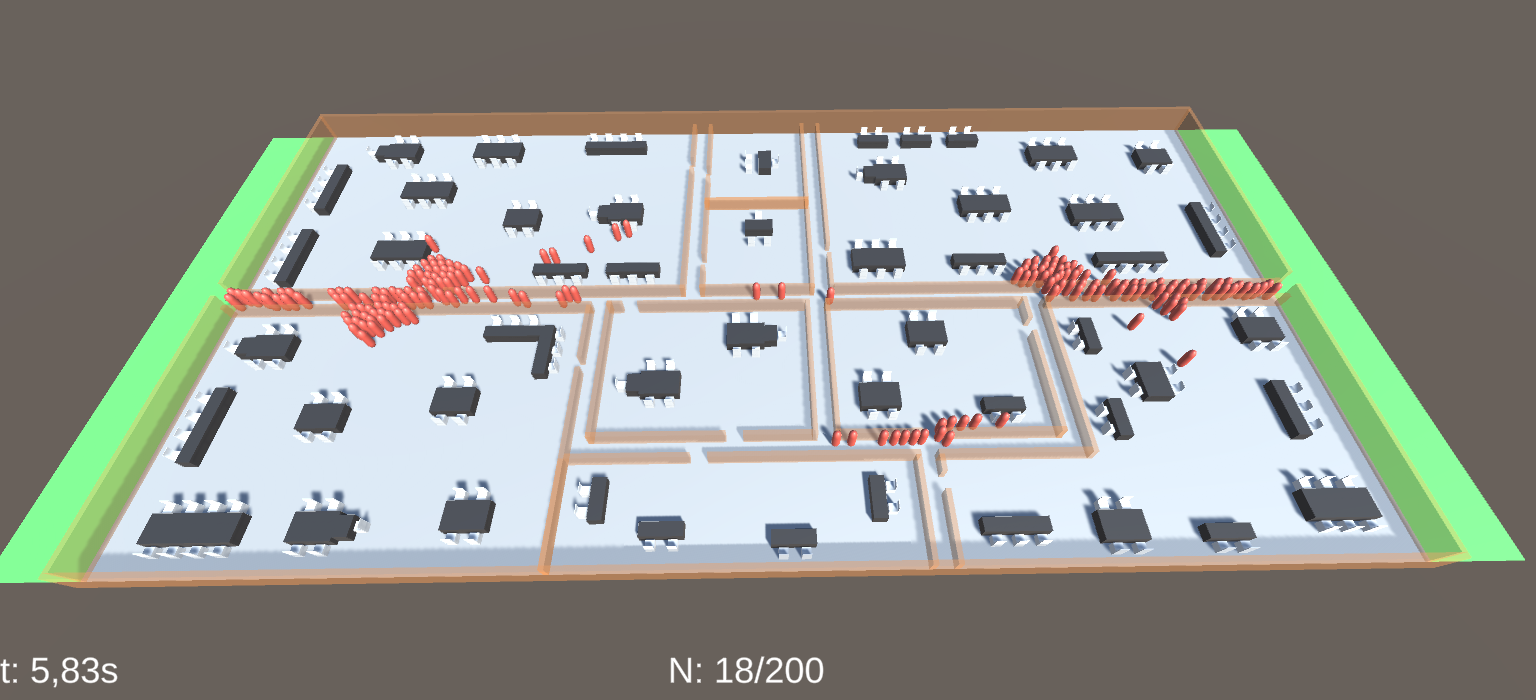
\includegraphics[scale=0.17]{1. couloir 1m -(2).png}
    
    \item 2. Temps moyen de dernière sortie : 28.96 sec
    \newline Temps max de dernière sortie : 33.6 sec
    \newline
    Il est très intéressant de voir qu'augmenter la taille du couloir a finalement eu un effet néfaste sur le temps de sortie
    ceci s'explique par deux facteurs :
    \newline
    $\hspace*{0.2cm}$- Les portes n'ont pas augmenter de taille
    \newline
    $\hspace*{0.2cm}$- Les personnes se retrouvent alors bloqué devant la porte de sortie (il ya génération d'un important flux devant
    les portes de sortie).
    \newline
    Donc il semble important que la taille des portes soit en adéquation avec la taille des couloirs avant de ne pas générer des flux trop important
    ci-dessous on peut voir les flux devant les portes de sorties.
    \newline 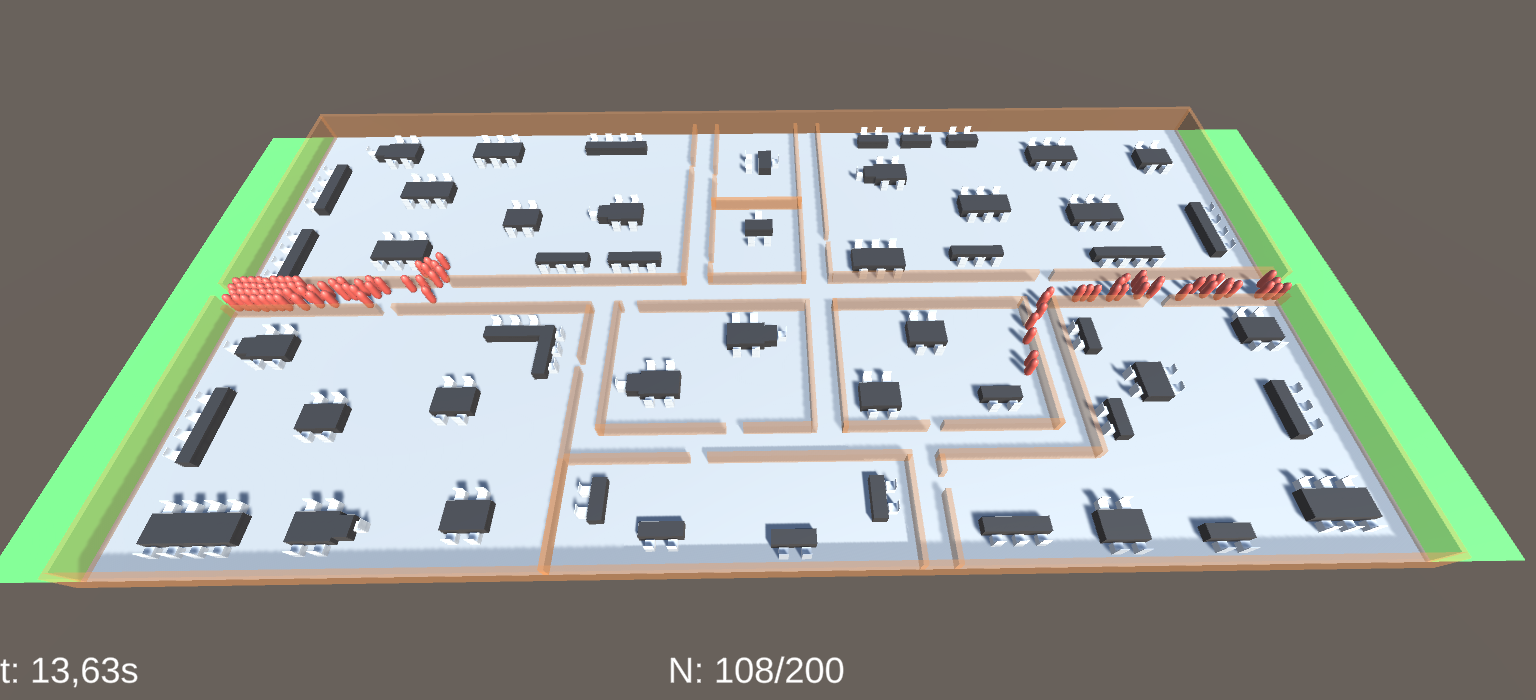
\includegraphics[scale=0.17]{2. couloir 1m50.png}

    \item 2. Temps moyen de dernière sortie : -
    \newline Temps max de dernière sortie : -
    \newline
    Pour ce problème j'ai simplement changer le couloir principal en le repassant à 1m de largeur (soit la largeur de la porte de sortie).
    Ceci étant pour tester si le majeur problème du 2. était le fait qu'il y avait des flux importants devant les portes de sorties du au faite que les couloirs
    était plus grand que les portes. Cependant j'ai laissé les autres couloirs à 1m50 afin de voir si cela avait une influence sur le temps de sortie moyen.
    \newline
    On a toujours les problèmes de flux importants devant les portes (cela bloque la fluidité de l'évacuation)(voir photo du 1.)

\end{itemize}

\end{document}